%!TEX root = Main.tex
\subsection*{Feature Extraction}
When doing speaker recognition it is advantageous to classify on the basis of extracted features from speech data, rather than the audio samples themselves \cite{Springer:36}.
Features were extracted on a frame-to-frame basis.
This was done on the assumption of pseudo-stationarity of human speech in the scale of a few tens of ms \cite{Springer:36}.
The frames consisted of 256 samples, with a new frame staring every 100 samples.
This means that we have a frame length of
\begin{equation}
t_{frame length} = \dfrac{N_{frame}}{F_s} = \dfrac{256}{48\ kHz} = 5.33\ ms
\end{equation}

and a frame interval of
\begin{equation}
t_{frame interval} = \dfrac{N_{interval}}{F_s} = \dfrac{100}{48\ kHz} = 2.08\ ms
\end{equation}

The features extracted for use in classification were $12^{th}$ order Mel-frequency Cepstral Coefficients (MFCC), as they hava proven effective in speaker regocnition applications and speech processing in general.
Further, so-called delta and double-delta coeffcients, the temporal derivatives $ \frac{dC}{dt} $ and double-derivatives $\frac{d^2C}{dt}$ of the MFCCs respectively, are used as features.
\footnote{For more on MFCC and feature extraction, see Appendix} \fxnote{fix footnotes}

\begin{figure}[H]
\centering
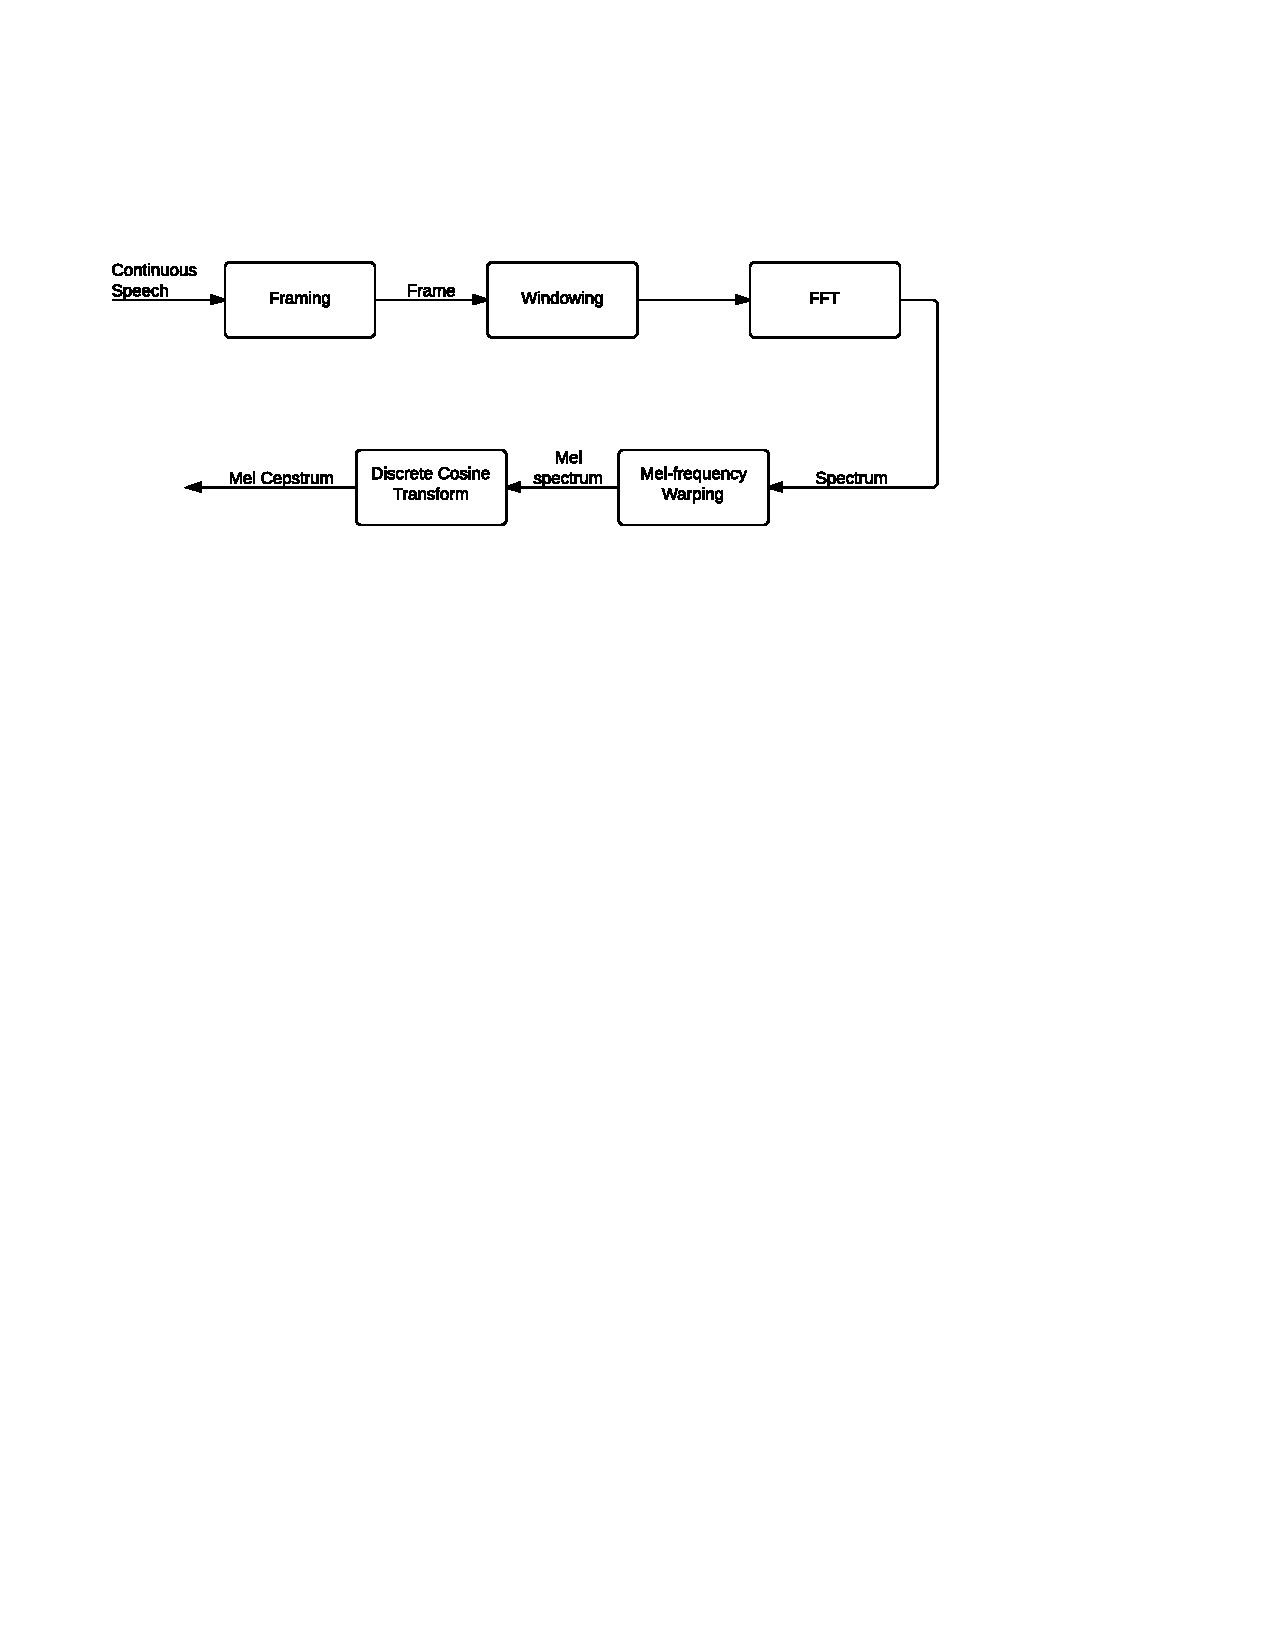
\includegraphics[width=0.7\linewidth]{MFCC_Flowchart_CROP}
\caption{Process for calculating MFCC}
\label{fig:MFCC_Flowchart}
\end{figure}
